\subsubsection{2D Samples of 3D Finger Knuckle Database}

First experiment on the database is to use the one session 190 subjects image to fine-tune models and then to test on the another session 190 subjects. It has $190*6$ genuine matching scores and $190*189*6$ imposter matching scores. From the result, we can see that these RFN-128-WRS, RFN-128-WS, EfficientNet can get very high matching accuracy. Meanwhile, the RFN-WRS has the minimal EER value among these models. As for the FKNet performance, it gets a very bad result on the 2D images of 3D finger knuckle. I think I have fully trained the FKNet. Maybe the model is overfitting on the training dataset. Updated ROC Curve and CMC Curve with RFNet, EfficientNet and DeConvRFNet. And each model with WRS is better than WS. \textcolor{red}{For the ROC curve, I add EfficientNetV2-S model performance.}

\begin{figure}[H]
	\centering
	\begin{subfigure}[b]{0.8\linewidth}
		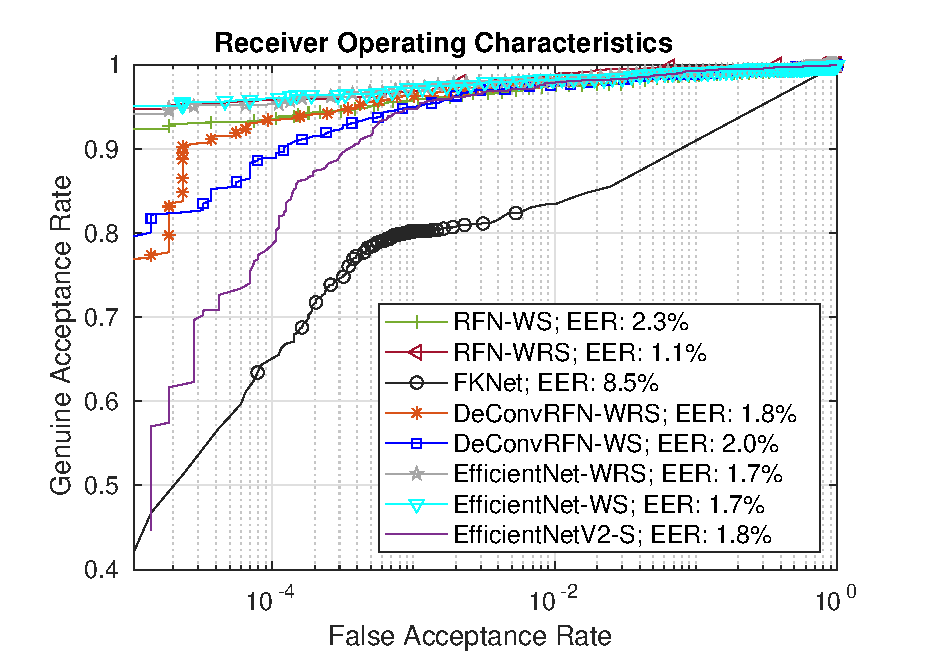
\includegraphics[width=\linewidth]{Figures/add-efficientv2-s/3d1s-2d-roc_compare_new.eps}
	\end{subfigure}
	\begin{subfigure}[b]{0.8\linewidth}
		\includegraphics[width=\linewidth]{Figures/fknet/3d1s-2d-cmc.eps}
	\end{subfigure}
\end{figure}


And then use the two session protocol. I use the rest samples of session1, and it has 191-228 subjects. In this kind of situation, the training dataset is too small. The two session protocol will test on the 190 subjects, these subjects can offer two session samples. Due to the training set is too small, so the matching performance is not very good. As for the FKNet, it cannot fit on two session protocol due to classification task.
\begin{figure}[H]
    \centering
    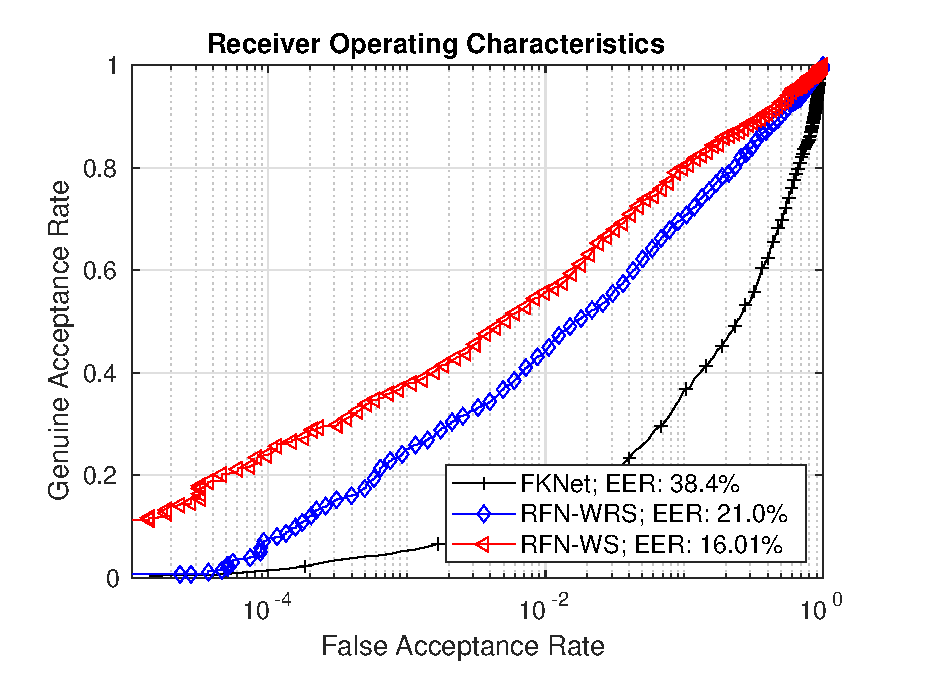
\includegraphics[width=0.8\linewidth]{Figures/fknet/two-3d1s-roc_compare_new.eps}
\end{figure}
